\documentclass[xcolor=table]{beamer}
\usepackage{verbatim}
\usepackage{default}
\usepackage{array}
\usepackage{makecell}
\usepackage{color, colortbl}

\beamertemplatenavigationsymbolsempty
\setbeamertemplate{footline}[frame number]

\renewcommand{\tt}{$ t\overline{t}\ $}
\newcommand{\ttz}{$ t\overline{t}Z\ $}
\newcommand{\tth}{$ t\overline{t}H\ $}

\definecolor{maroon}{cmyk}{0,0.87,0.68,0.32}

\setbeamersize{text margin left=5mm} 

\begin{document}
\begin{frame}{Current status}

\begin{itemize}
\item Existing inclusive $t\bar{t}$ sample, including mass and width variations: 436M events
\begin{itemize}
\item Nevertheless, MC statistics is scarce
\begin{itemize}
\item ~200 MC events in 10j4b $l$+jets category
\item ~140 MC events in 8j4j $l^+l^-$+jets category
\end{itemize} 
\item Need factor of 10 increase in statistics to ensure fit stability in the sensitive high multiplicity/high discriminant region
\item This requires the development of a gen level filter for efficient MC production
\end{itemize}
\end{itemize}
\begin{itemize}
\item Various filter configurations have been studied and we have a preferred configuration
\end{itemize}
\begin{itemize}
\item MC production can be started once new release is available
\item Backport and genfragment are available \\(Thanks Javier Fernandez!)
\item CMSSW modification are signed by generator conveners \\(Thanks L.Perrozzi!)
\item Currently waiting for new cmssw build containing the backport
\begin{itemize}
\item New patch release has to be issued by release managers
\end{itemize}
\end{itemize}
%\begin{center}
%{\tiny \begin{tabular}{|c|c|c|c|c|c|}
%\hline Filter cuts & Filter eff. & Bias\footnote{Fraction of events passing offline cuts but rejected by gen filter} ($N_J^{rec}=8$) &  ($N_J^{rec}=9$)&  ($N_J^{rec}>=10$)&  Sample ($\times 10$) \\ 
%\hline \thead{HT$>$500} & $0.12\pm 0.0008$ & 0.018 & 0.013 & 0.006 & 516M \\ 
%\hline \thead{nJets+nLep$>$=8} & $0.04 \pm 0.0005$ & 0.087 & 0.03 & 0.006 & 172 M\\ 
%\hline \thead{HT$>$500 \\  nJets+nLep$>$=8} & $0.026 \pm 0.0004$  & 0.09 & 0.03 & 0.01 & 112 M\\ 
%\hline 
%\end{tabular} }
%\end{center}
\end{frame}

\begin{frame}{Two scenarios for new filtered samples}
\begin{itemize}
\item Two independent samples with different lepton and jet multiplicity cuts:
\begin{itemize}
\item Optimal for the two channels
\item Uses gen level cuts which are probably not useful for other analyses
\end{itemize}
\vspace{10pt}
\item Common sample with no fully hadronic $t\bar{t}$ decays
\begin{itemize}
\item Potentially useful for other analyses
\item Worse filter efficiency
\end{itemize}
\end{itemize}
\vspace{25pt}
\hrule
\begin{itemize}
\item Filter efficiency and acceptance loss were calculated on /MINIAODSIM level
\item Efficiency values were verified using actual filter implementation in small private /GEN-SIM production 
\end{itemize}
\end{frame}

\begin{frame}{Filters summary  (l+jets and OS)}
\begin{itemize}
\item{\footnotesize  Preferred configuration: $HT>500,\, \mathrm{nJets+nLep}\geq8,\,  \mathrm{nLep}\geq1$ (26M)}
\end{itemize}
\vspace{-19pt}
\begin{center}
{\tiny \begin{tabular}{|c|c|c|c|c|c|c|}
            \cline{1-7}
             & & \multicolumn{5}{|c|}{Acceptance loss in different jet multiplicity regions\footnote{Fraction of events passing offline cuts but rejected by gen filter}}\\
            \cline{1-7}
\hline Filter cuts & Filter eff. $\times 10^{-2}$ & OS $N_J=7$& OS $N_J\geq8$ & SL $N_J=9$& SL $N_J>9$& Ext ($\times 10$) \\ 
\hline \thead{{\tiny HT$>$500} \\ {\tiny  nJets+nLep$\geq$6} \\ {\tiny $\geq1$ lepton}} & $2.3 \pm 0.03$  & --- & --- & --- & --- & 100 M\\
\hline \thead{{\tiny HT$>$500} \\ {\tiny  nJets+nLep$\geq$7} \\ {\tiny $\geq1$ lepton}} & $1.4 \pm 0.02$  & 0.04 & 0.02 & --- & --- & 61 M\\
\hline \rowcolor{lightgray} {\tiny \thead{ HT$>$500 \\ nJets+nLep$\geq$8 \\  $\geq1$ lepton}} & $0.6 \pm 0.02$  & 0.14 & 0.04 & 0.11 & 0.08 & 26 M\\ 
\hline \thead{{\tiny HT$>$500} \\ {\tiny nJets+nLep$\geq$9} \\ {\tiny $\geq1$ lepton}} & $0.2 \pm 0.01$   & 0.43 & 0.14 & 0.19 & 0.1 & 9M\\ 
\hline \thead{{\tiny HT$>$500} \\ {\tiny nJets+nLep$\geq$10} \\ {\tiny $\geq1$ lepton}} & $0.08 \pm 0.007$   & --- & --- & --- & 0.19 & 3.5M\\
\hline 
\end{tabular} }
\end{center}
\end{frame}

\begin{frame}{Filter optimized for l+jets channel}
\begin{itemize}
\item{\footnotesize  Preferred configuration: $HT>500,\, \mathrm{nJets+nLep}\geq9,\, \mathrm{nLep}=1$ (9M)}
\end{itemize}
\begin{center}
{\tiny \begin{tabular}{|c|c|c|c|c|}
            \cline{1-5}
             & & \multicolumn{3}{|c|}{Acceptance loss in different jet multiplicity regions\footnote{Fraction of events passing offline cuts but rejected by gen filter}}\\
            \cline{1-5}
\hline Filter cuts & Filter eff. & SL ($N_J^{rec}=9$)& SL ($N_J^{rec}>9$)&  Ext ($\times 10$) \\ 
\hline \thead{HT$>$500 \\  nJets+nLep $\geq$8 \\  $1$ lepton} & $0.005 \pm 0.0002$  & 0.11 & 0.08 & 21.8 M\\ 
\hline \rowcolor{lightgray}\thead{HT $>$ 500 \\  nJets+nLep $\geq\phantom{M}$9 \\  $1$ lepton} & $0.002 \pm 0.0001$  & 0.19 & 0.10 & 8.7M\\
\hline \thead{HT$>$500 \\  nJets+nLep$>$=10 \\  $1$ lepton} & $0.0007 \pm 6.5\times 10^{-5}$  & --- & 0.19 & 3M\\
\hline 
\end{tabular} }
\end{center}

\end{frame}

\begin{frame}{Filter optimized for OS dilpeton channel}
\begin{itemize}
\item{\footnotesize  Preferred configuration: $HT>500,\, \mathrm{nJets+nLep}\geq7,\,  \mathrm{nLep}=2$ (9M)}
\end{itemize}
\begin{center}
{\tiny \begin{tabular}{|c|c|c|c|c|}
            \cline{1-5}
             & & \multicolumn{3}{|c|}{Acceptance loss in different jet multiplicity regions\footnote{Fraction of events passing offline cuts but rejected by gen filter}}\\
            \cline{1-5}
\hline Filter cuts 	& Filter eff. 	& OS  ($N_J^{rec}=7$)& OS ($N_J^{rec}\geq8$)&  Ext ($\times 10$) \\
\hline \thead{HT$>$500 \\  nJets+nLep$>$=5 \\  $2$ lepton} & $0.0046 \pm 5.5e-05$  & 0.21 & 0.23 & 20 M\\ 
\hline \thead{HT$>$500 \\  nJets+nLep$>$=6 \\  $2$ lepton} & $0.0033 \pm 4.7e-05$  & 0.21 & 0.23 & 14.4 M\\
\hline \rowcolor{lightgray} \thead{HT$>$500 \\  nJets+nLep$>$=7 \\  $2$ lepton} & $0.0020 \pm 3.6e-05$  & 0.23 & 0.24 & 8.7 M\\ 
\hline \thead{HT$>$500 \\  nJets+nLep$>$=8 \\  $2$ lepton} & $0.0009 \pm 2.4e-05$  & 0.31 & 0.25 & 3.9 M\\
\hline 
\end{tabular} }
\end{center}

\end{frame}

\begin{frame}{Summary}
\begin{itemize}
\item \underline{There are two options to get 10$\times$ MC stat extension:}
\begin{itemize}
\item (Preferred) Two samples with different gen level cuts\\ (Total of 18M events passing the filters):
\begin{itemize}
\item OS \textbf{9M events}: $HT>500, nJets+nLep\geq7, nLep=2$
\item SL \textbf{9M events}: $HT>500, nJets+nLep\geq9, nLep=1$
\end{itemize}
\item Combined sample\\ (Total of 26M events passing the combined filter):
\begin{itemize}
\item SL+OS: $HT>500, nJets+nLep\geq8, nLep\geq1$
\end{itemize}
\end{itemize}
\end{itemize}
\end{frame}

\begin{frame}{Definitions}

\begin{itemize}
\item Variable definitions:
\begin{itemize}
\item $HT=\sum\limits_{j:p_T>30,|\eta|<2.4} {p_T(j)}$
\item nJets= number of gen jets with $p_T>30$\\
No $\eta(j)$ cut due to different CMSSW filter logic.
\item Jets in HT and multiplicity definition may include jets from isolated leptons
\end{itemize}
\item Lepton cuts are applied using LHE filter, similar to NoFullyHadronicDecays filter applied to single-top MC samples
\end{itemize}

\end{frame}
% % % % % % % % % % % % % % % % % % %
%
%\begin{frame}{Bias from HT cut (MVA). 8 jet bin}
%\vspace{-5pt}
%\begin{figure}
%\centering
%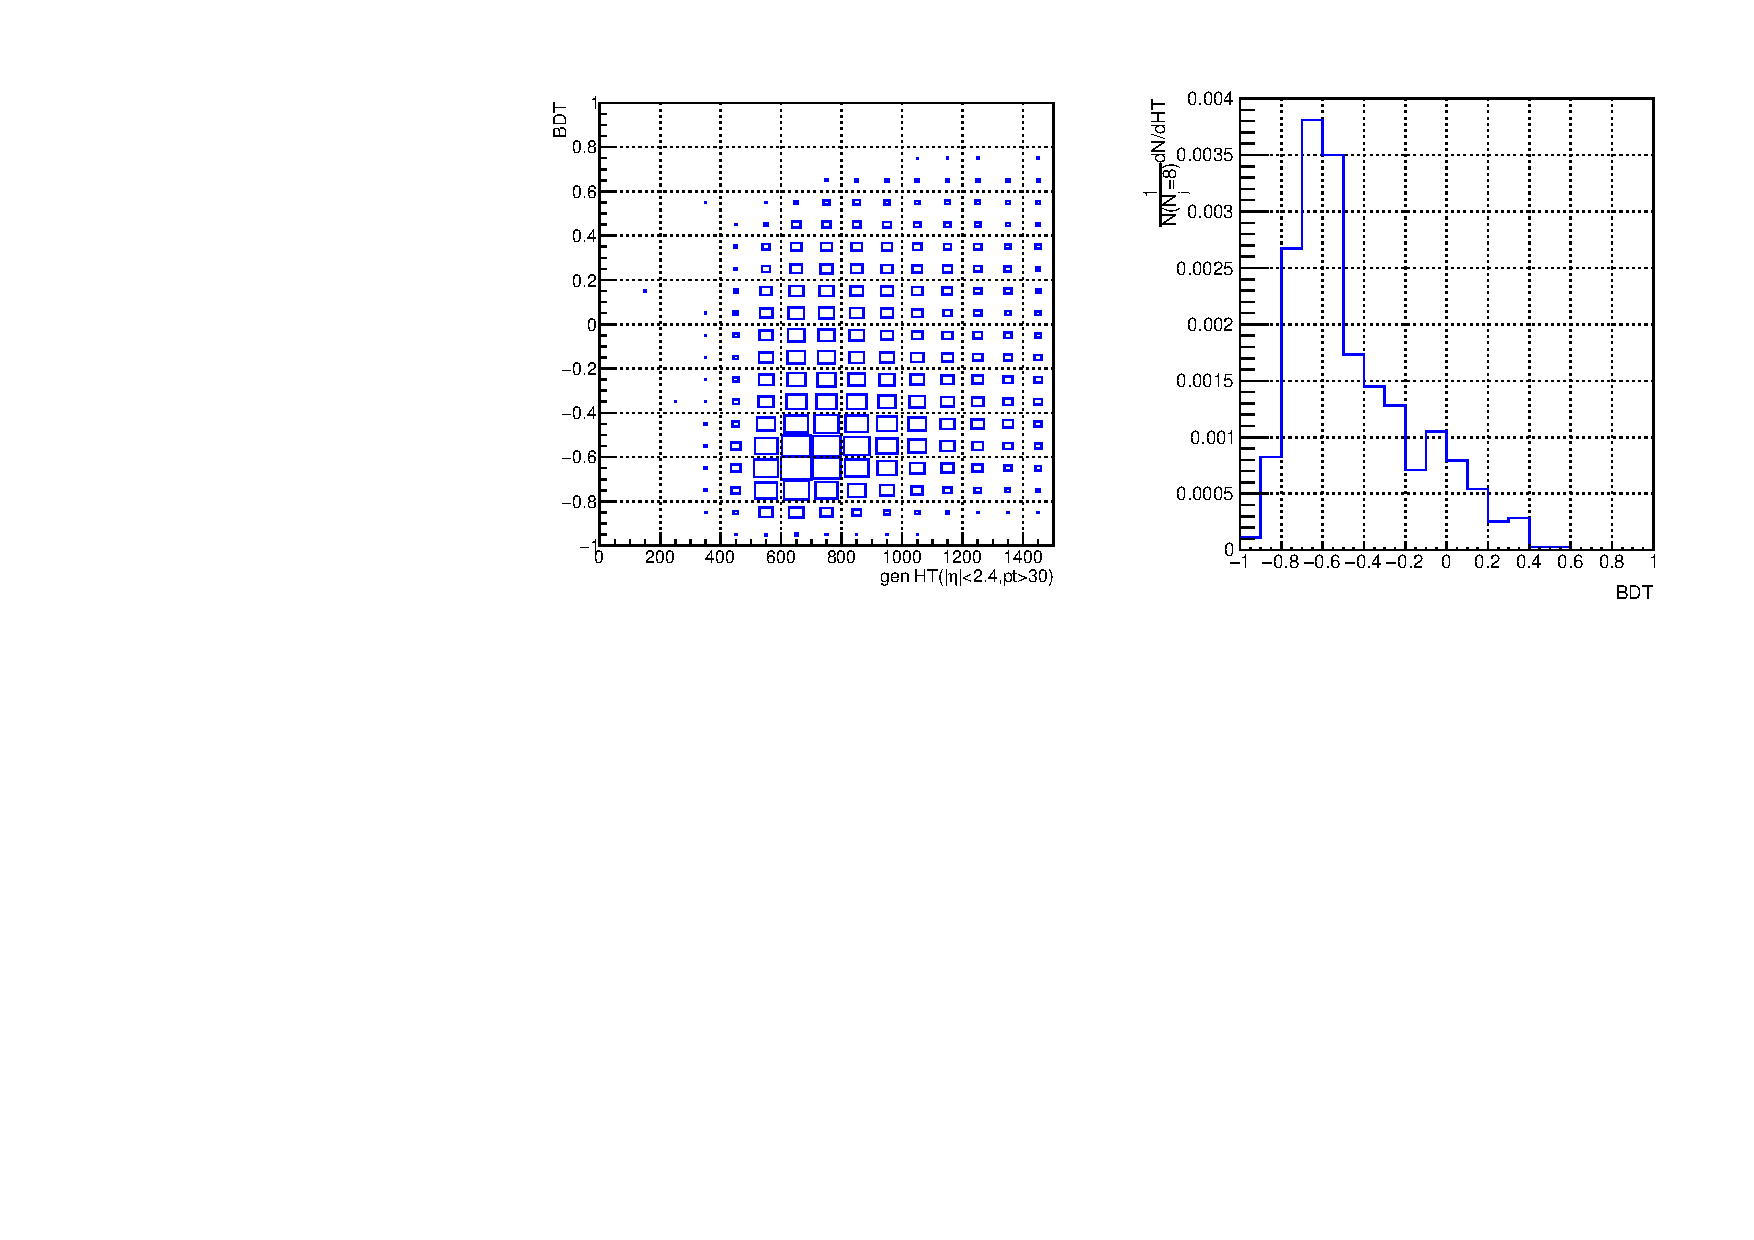
\includegraphics[height=0.55\textheight]{./materials/8j/CMS4}
%\caption{{\tiny (Left) Correlation of reconstructed and generator-level observables. (Right) Spectrum of tt background events that do not pass gen-level HT cut.} }
%\label{fig:CMS4}
%\end{figure}\vspace{-15pt}
%{\small \begin{itemize}
%\item Gen cut introduces small bias in acceptance estimation
%\end{itemize}}
%\end{frame}
%
%\begin{frame}{Bias from HT and mult cut (MVA). 8 jet bin}
%\vspace{-5pt}
%\begin{figure}
%\centering
%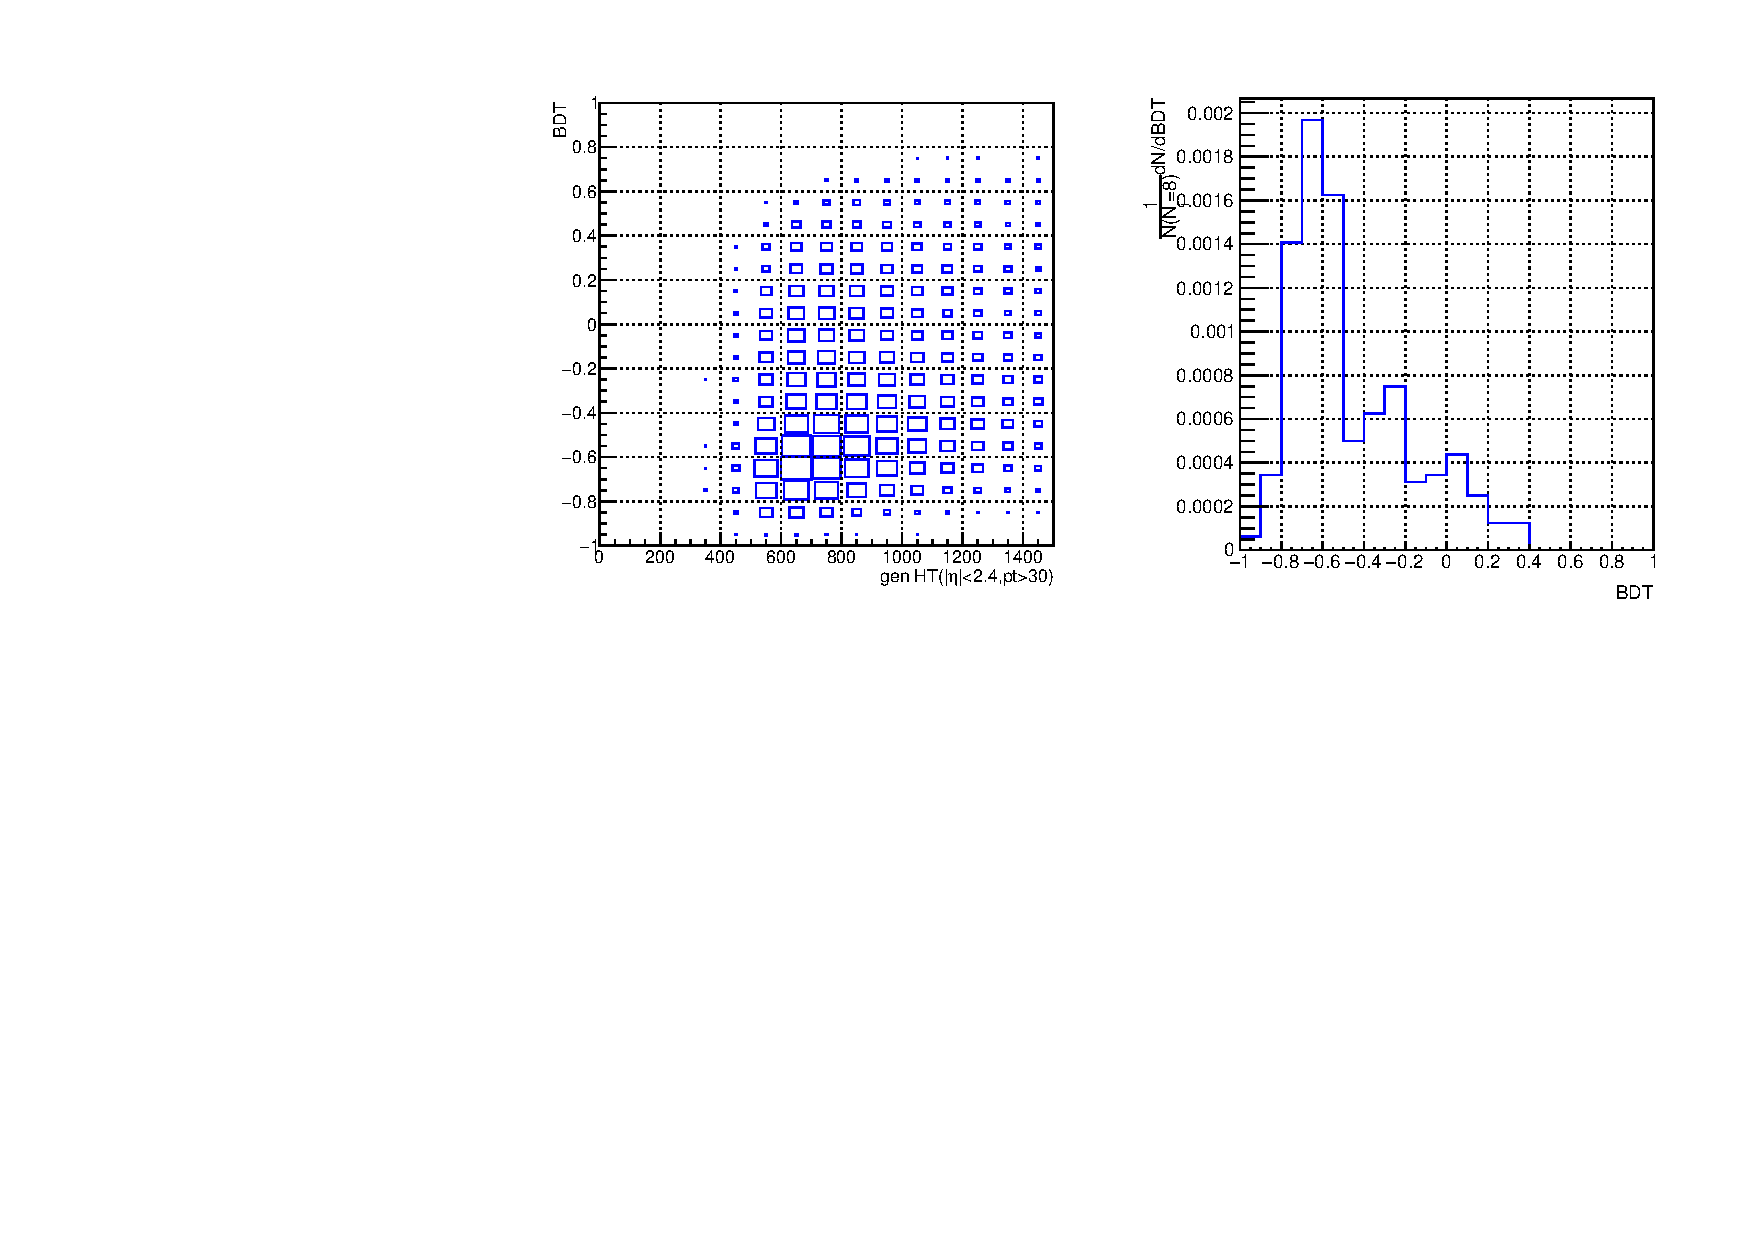
\includegraphics[height=0.55\textheight]{./materials/8j_htmult/CMS4}
%\caption{{\tiny (Left) Correlation of reconstructed and generator-level observables. (Right) Spectrum of tt background events that do not pass gen-level HT and multiplicity cut.} }
%\label{fig:CMS4}
%\end{figure}\vspace{-15pt}
%{\small \begin{itemize}
%\item {\small No clear pattern how gen multiplicity cut affects BDT.}
%\end{itemize}}
%\end{frame}
%% % % % % % % % % % % % % % % % % % %
%
%\begin{frame}{Bias from HT (MVA). 9 jet bin}
%\vspace{-5pt}
%\begin{figure}
%\centering
%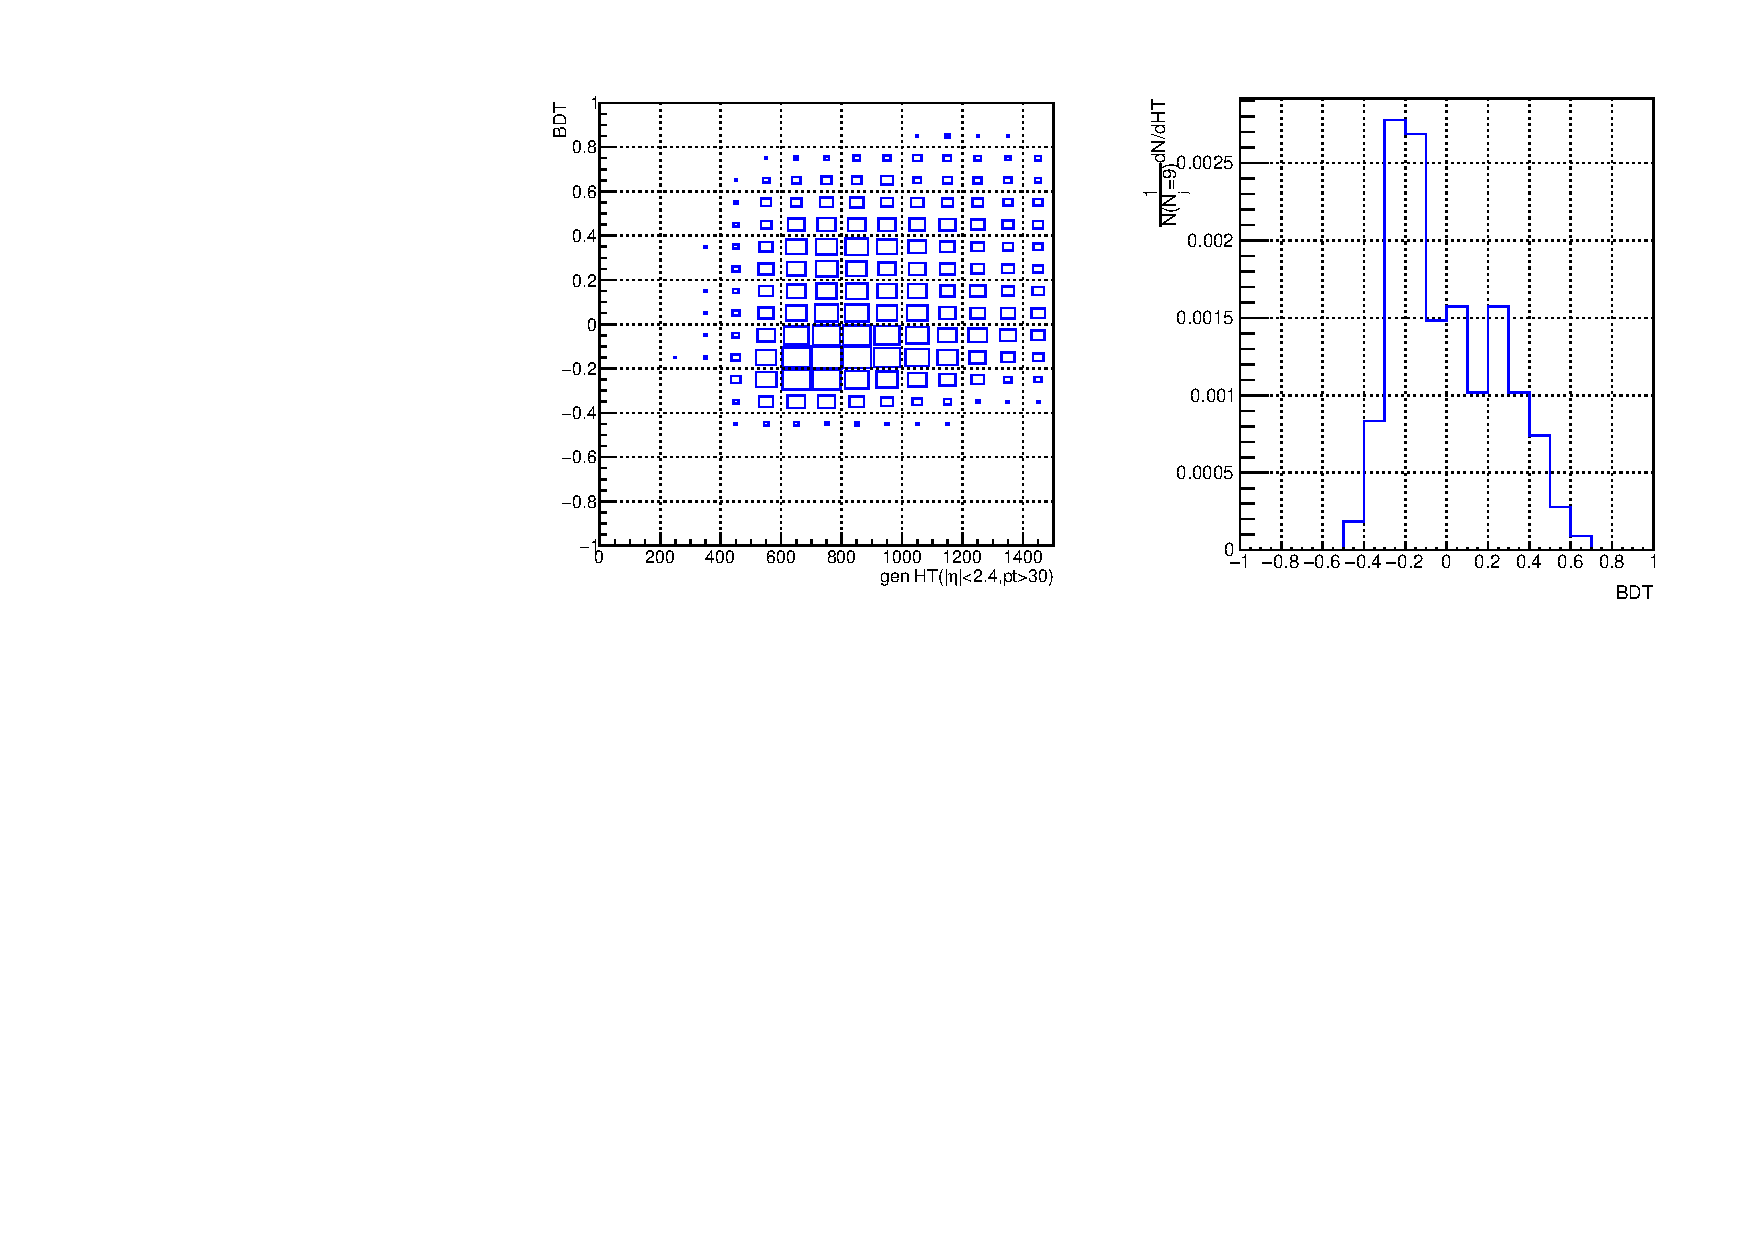
\includegraphics[height=0.55\textheight]{./materials/9j/CMS4}
%\caption{{\tiny (Left) Correlation of reconstructed and generator-level observables. (Right) Spectrum of tt background events that do not pass gen-level HT cut.} }
%\label{fig:CMS4}
%\end{figure}\vspace{-15pt}
%{\small \begin{itemize}
%\item Gen cut introduces small bias in acceptance estimation
%\end{itemize}}
%\end{frame}
%
%\begin{frame}{Bias from HT and mult cut (MVA). 9 jet bin}
%\vspace{-5pt}
%\begin{figure}
%\centering
%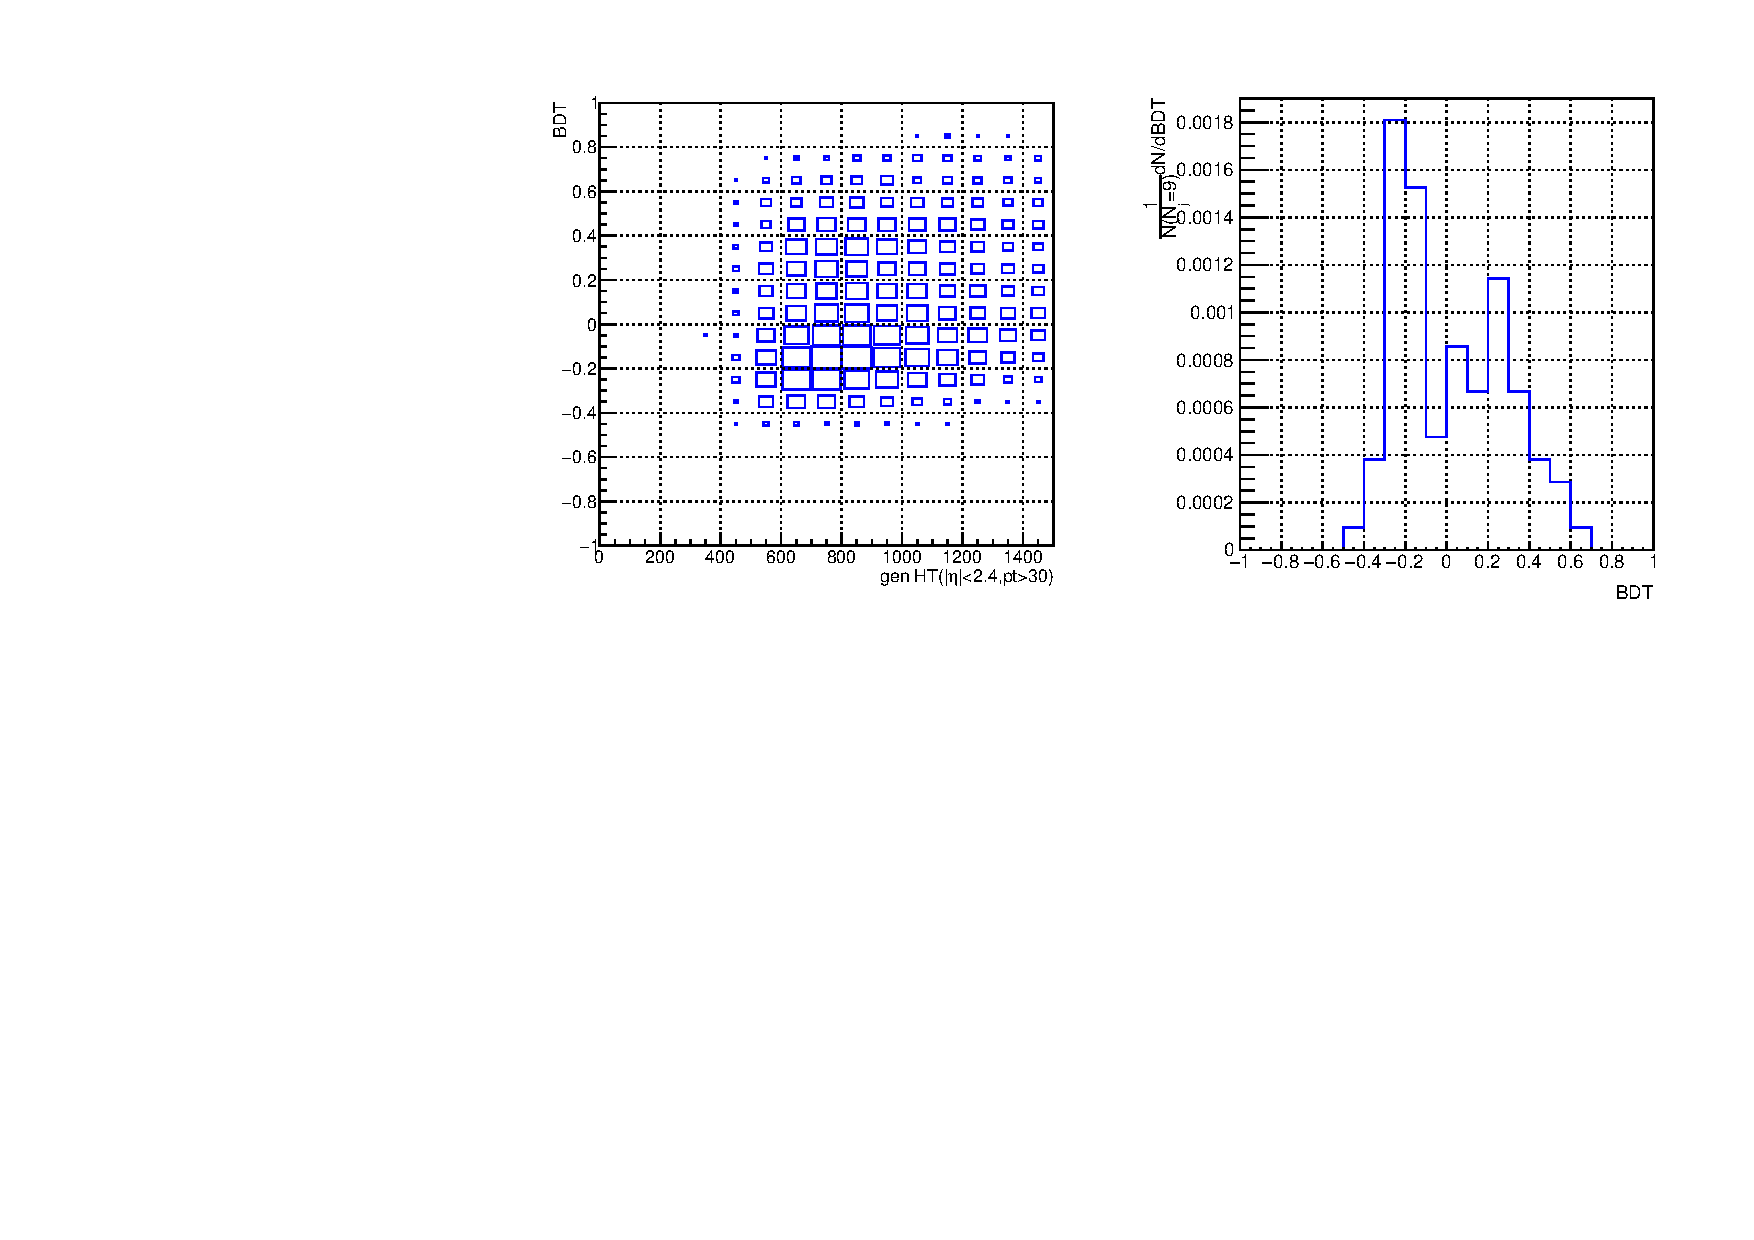
\includegraphics[height=0.55\textheight]{./materials/9j_htmult/CMS4}
%\caption{{\tiny (Left) Correlation of reconstructed and generator-level observables. (Right) Spectrum of tt background events that do not pass gen-level HT and multiplicity cut.} }
%\label{fig:CMS4}
%\end{figure}\vspace{-15pt}
%{\small \begin{itemize}
%\item {\small No clear pattern how gen multiplicity cut affects BDT.}
%\end{itemize}}
%\end{frame}
%% % % % % % % % % % % % % % % % % % %
%
%\begin{frame}{Bias from HT (MVA). 10+ jet bin}
%\vspace{-5pt}
%\begin{figure}
%\centering
%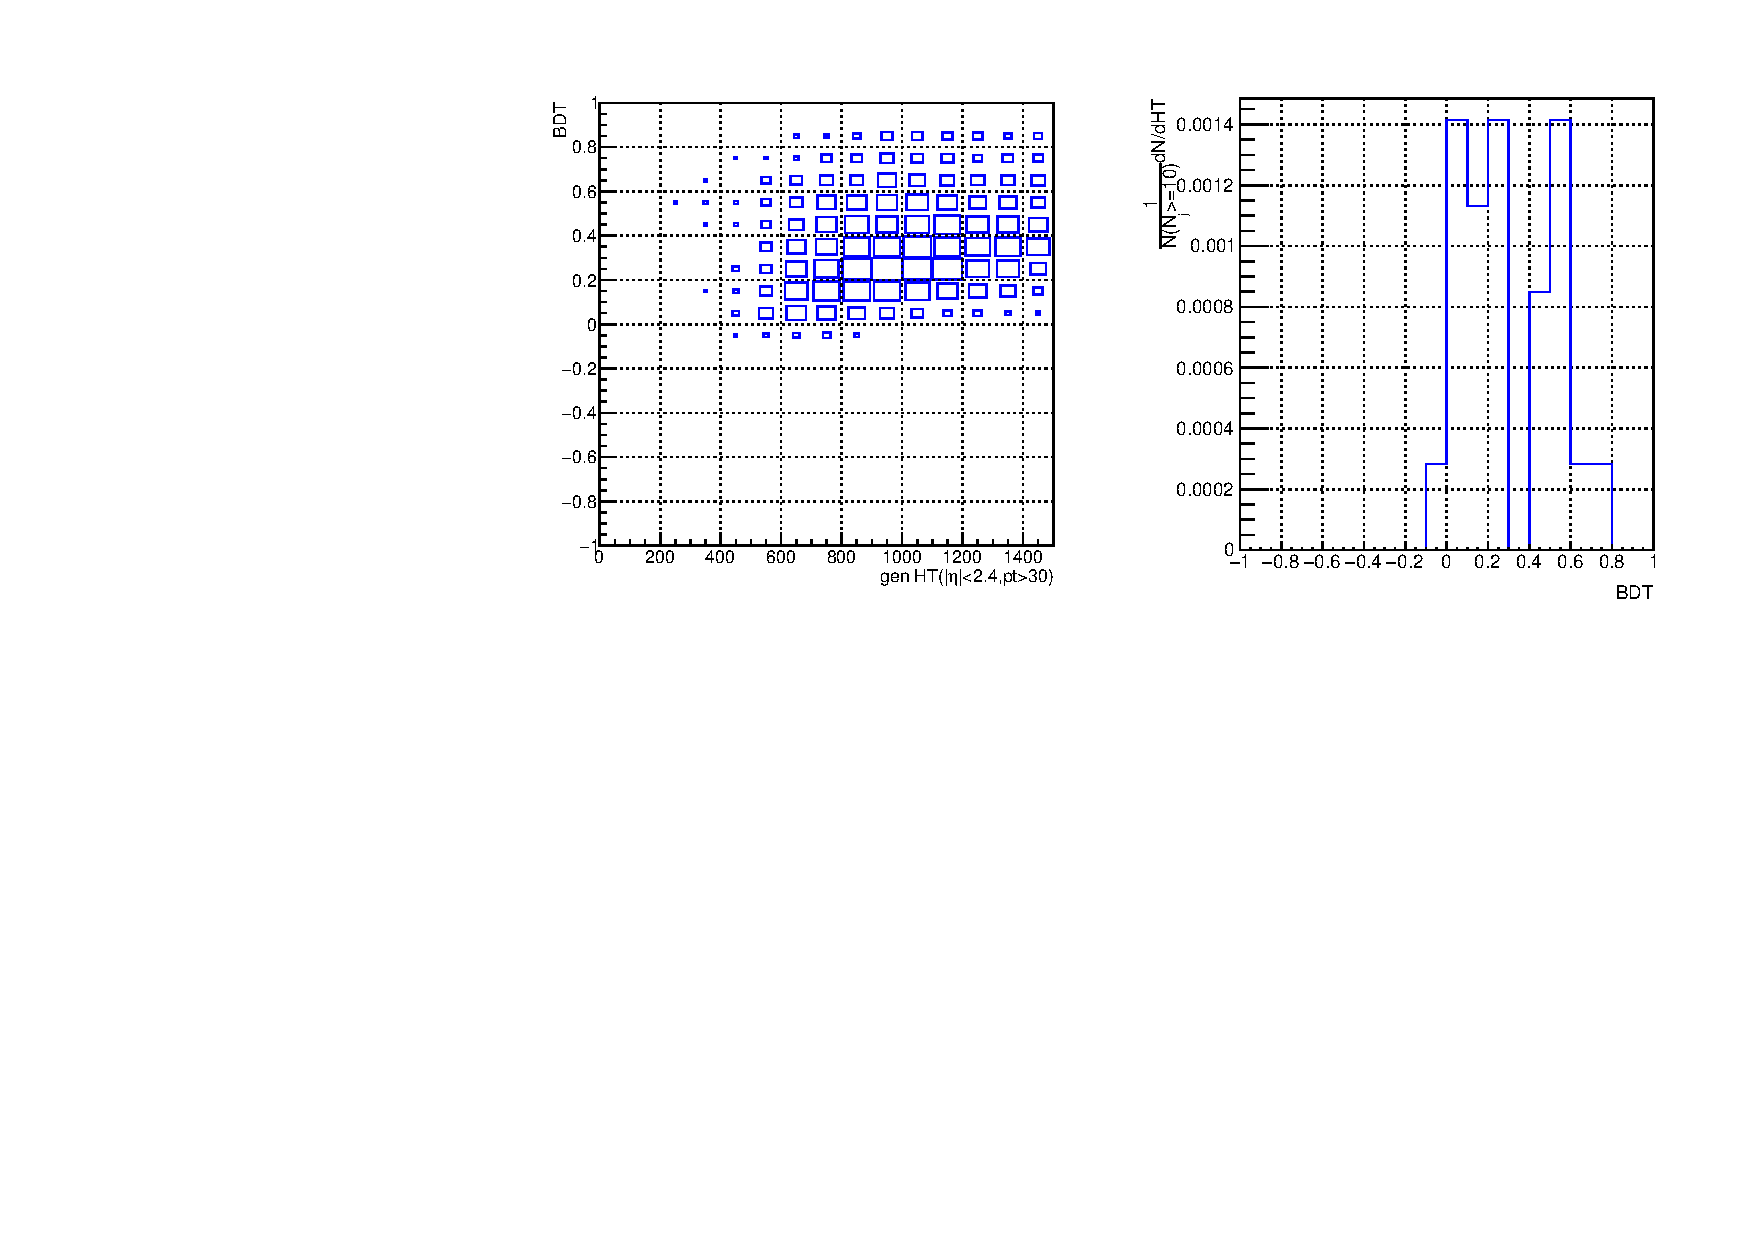
\includegraphics[height=0.55\textheight]{./materials/10j/CMS4}
%\caption{{\tiny (Left) Correlation of reconstructed and generator-level observables. (Right) Spectrum of tt background events that do not pass gen-level HT cut.} }
%\label{fig:CMS4}
%\end{figure}\vspace{-15pt}
%{\small \begin{itemize}
%\item {\tiny Almost vanishing bias from gen-level cut in high multiplicity categories.}
%\end{itemize}}
%\end{frame}
%
%\begin{frame}{Bias from HT and mult cut (MVA). 10+ jet bin}
%\vspace{-5pt}
%\begin{figure}
%\centering
%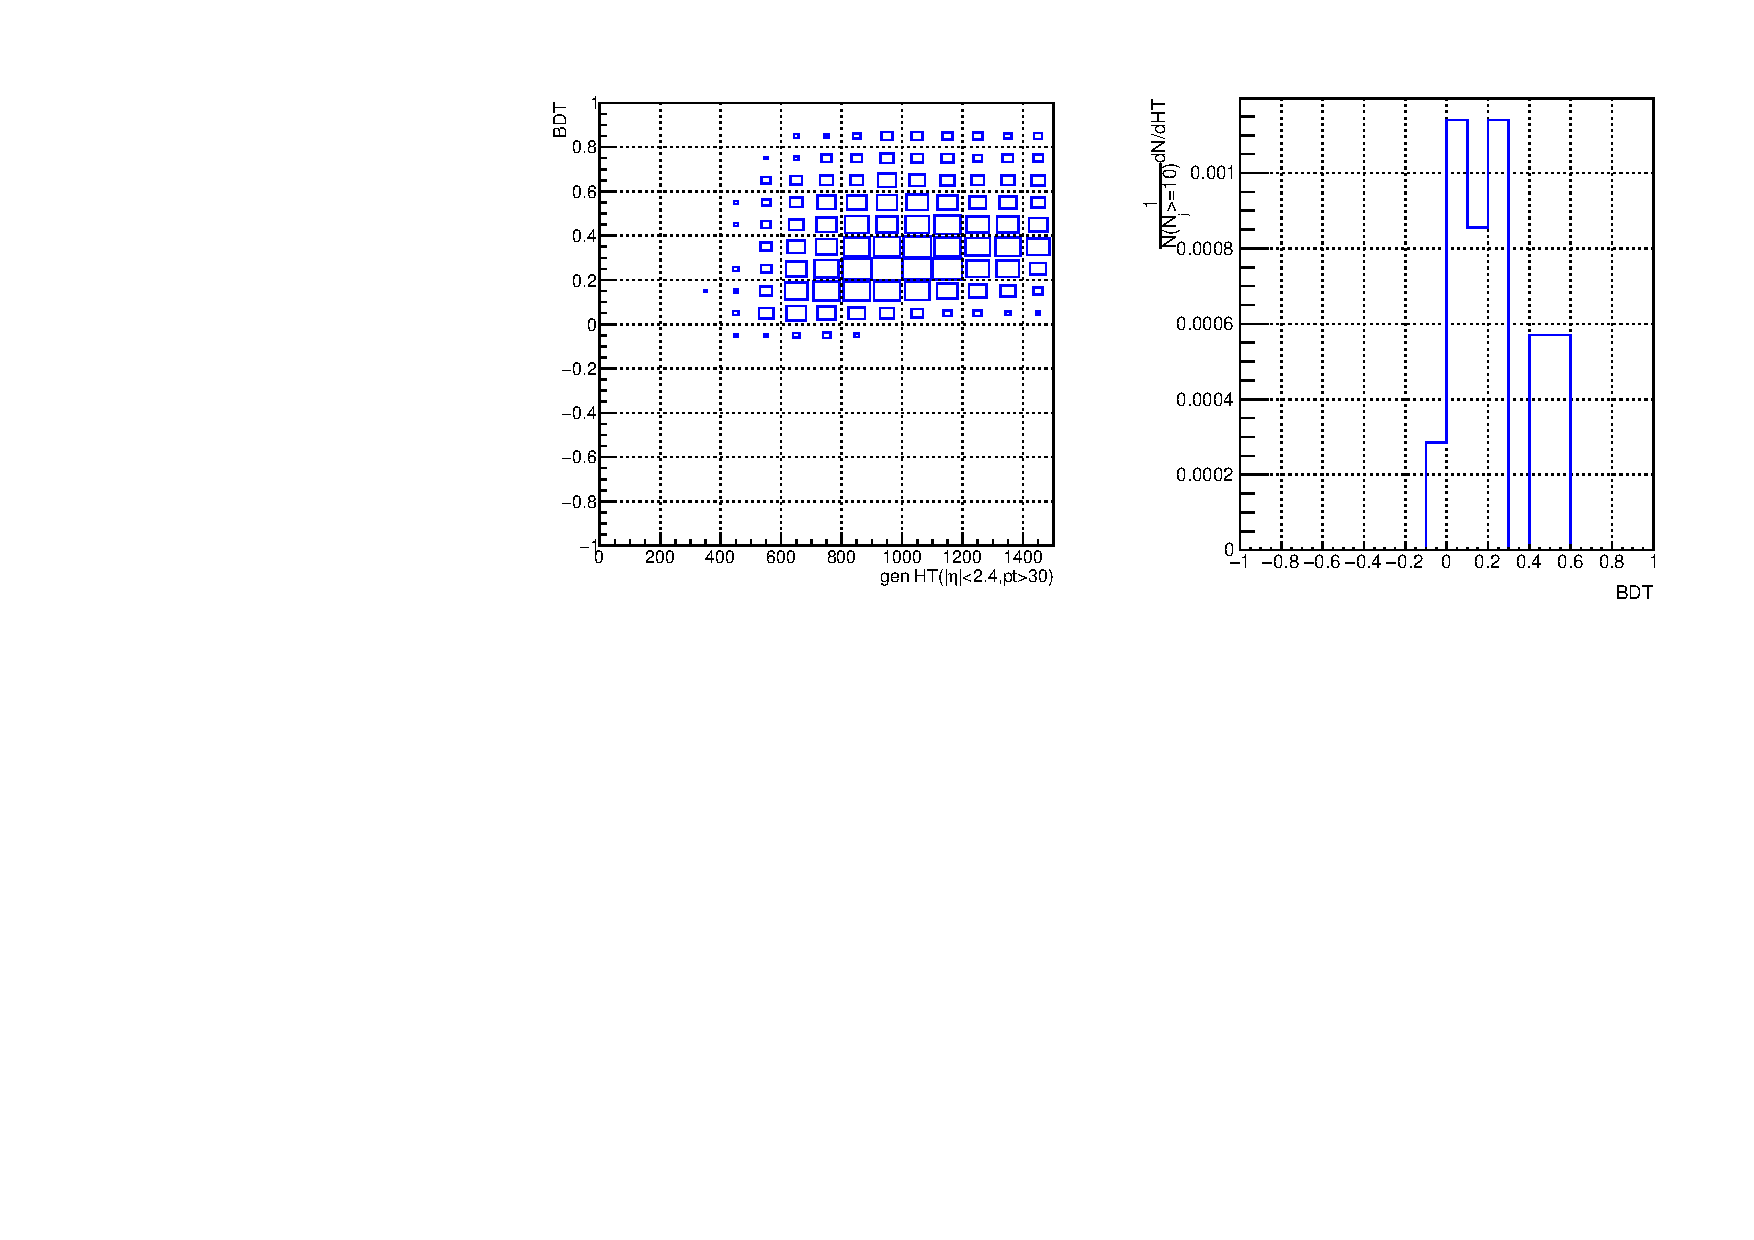
\includegraphics[height=0.55\textheight]{./materials/10j_htmult/CMS4}
%\caption{{\tiny (Left) Correlation of reconstructed and generator-level observables. (Right) Spectrum of tt background events that do not pass gen-level HT and multiplicity cut.} }
%\label{fig:CMS4}
%\end{figure}\vspace{-15pt}
%{\small \begin{itemize}
%\item {\small Larger bias for high MVA values.}
%\end{itemize}}
%\end{frame}
%
%\begin{frame}{}
%SlimmedGenJets info:
%https://twiki.cern.ch/twiki/bin/view/CMSPublic/WorkBookMiniAOD2016
%\\
%Filters:\\
%HT\\
%http://cmslxr.fnal.gov/source/GeneratorInterface/GenFilters/python/genHTFilter\_cfi.py\\
%http://cmslxr.fnal.gov/source/GeneratorInterface/GenFilters/interface/PythiaFilterHT.h\\
%\vspace{10pt}
%Jet multiplicity\\
%http://cmslxr.fnal.gov/source/GeneratorInterface/GenFilters/src/NJetsMC.cc
%\end{frame}
%
%
%\begin{frame}
%
%{\Huge BACKUP}
%
%\end{frame}
%
%\begin{frame}{Lepton transverse momentum}
%\begin{figure}
%\centering
%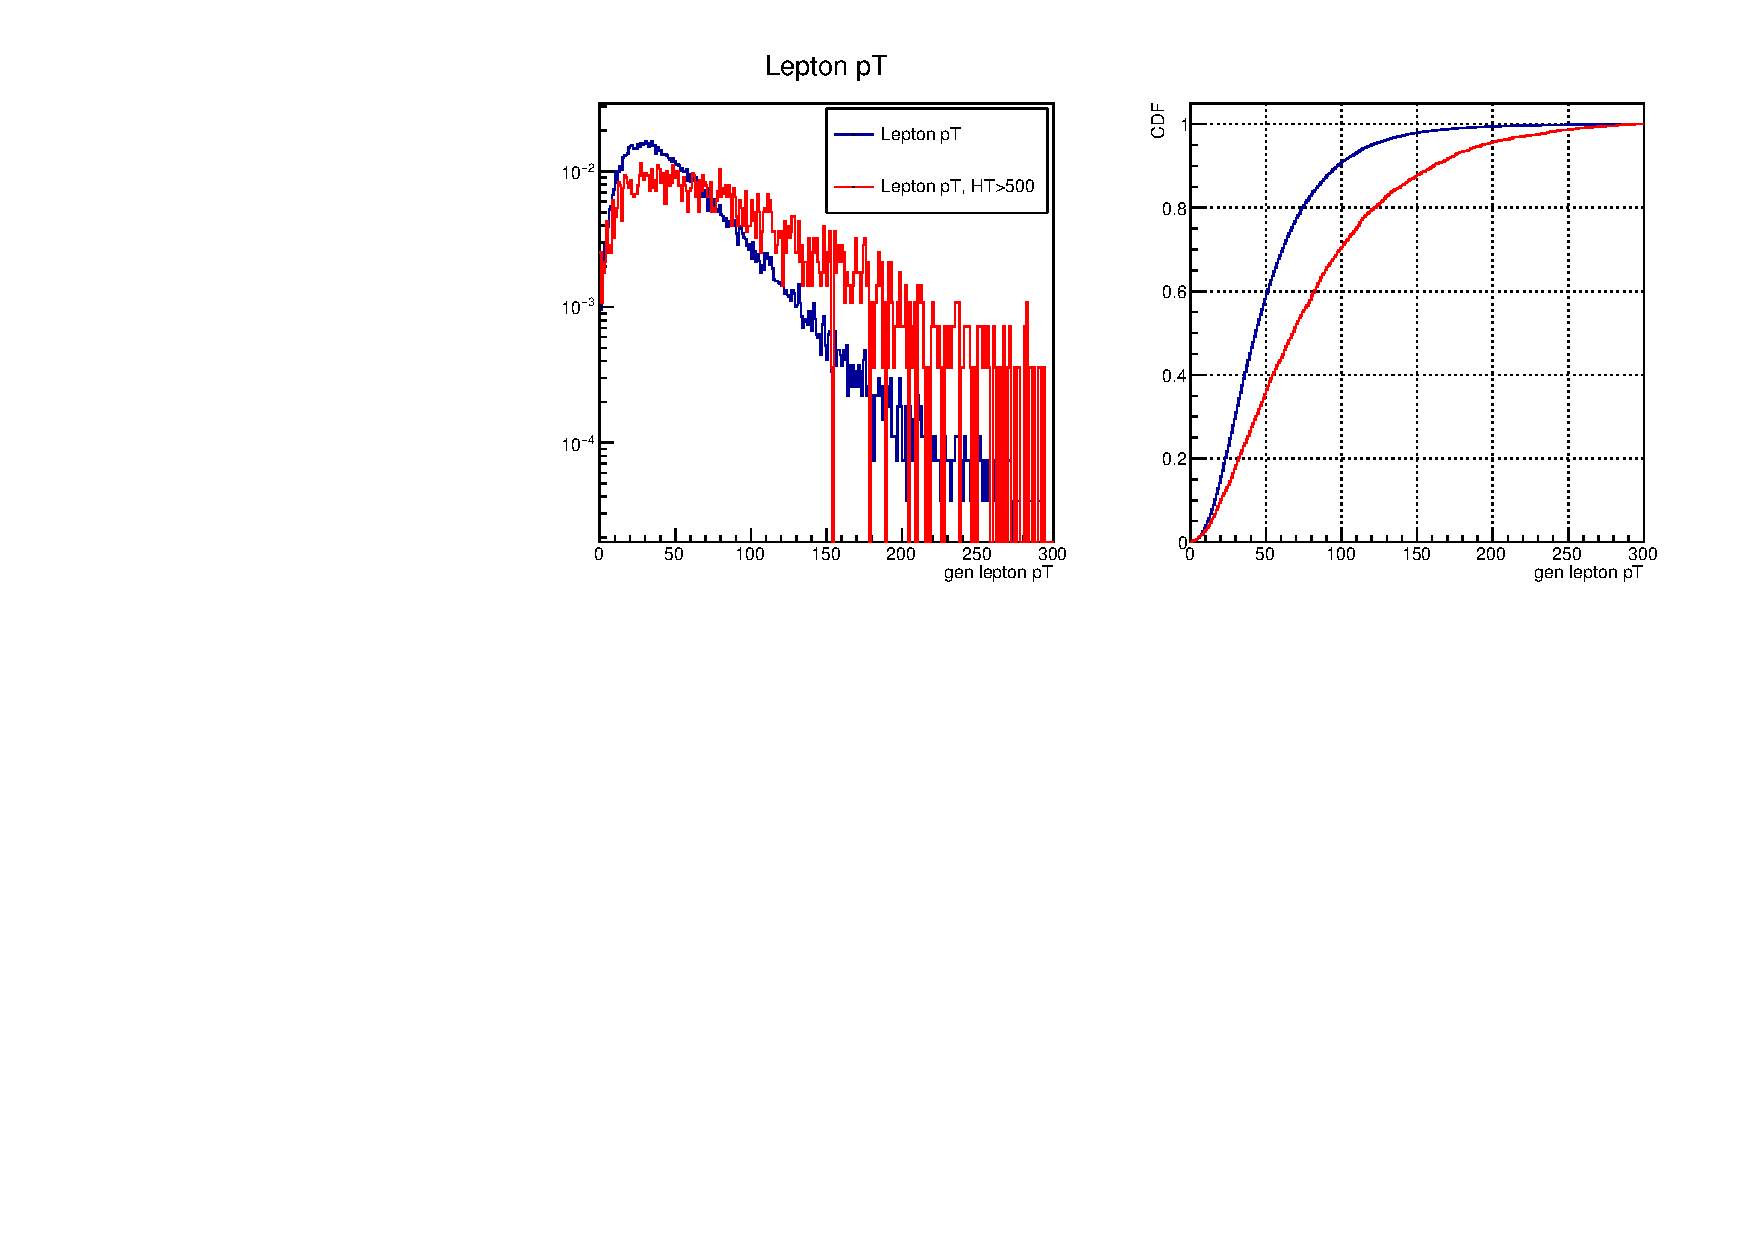
\includegraphics[width=\linewidth]{./materials/Lepton/CMS_Eff3}
%\caption{Comparison of generator level lepton transverse momentum}
%\label{fig:CMS_Eff3}
%\begin{itemize}
%\item Additional gen cut on lepton transverse momentum does not contribute much to overall gen filter efficiency
%\end{itemize}
%\end{figure}
%
%\end{frame}
%
%\begin{frame}{Samples and baseline selection}
%
%\begin{itemize}
%\item $\mu+$jets channel offline cuts:
%\begin{itemize}
%\item Only events passing offline selection (triggers + tight lepton + $\geq 6$ jets ($pT>30$, $|\eta|<2.4$) + $\geq 2$ medium tags + HT$>$500 + MET$>$50)
%\item At the generator level used \texttt{SlimmedGenJets} collection
%\end{itemize}
%\end{itemize}
%\end{frame}


\end{document}
